% http://www.idt.mdh.se/phd/thesis/kthesis-1.0/
\documentclass[a4paper,11pt]{kthesis}
\usepackage[T1]{fontenc}
\usepackage[normalem]{ulem}
\usepackage[english]{babel}
\usepackage{listings,babel}
\lstset{breaklines=true,basicstyle=\ttfamily}
\usepackage{graphicx}
\usepackage{moreverb}
\usepackage{float}
\usepackage{cite}

\title{A performance-driven SoC architecture for video synthesis}
\date{June 2010}
\type{Master of Science Thesis}
\department{Department of Software and Computer Systems}
\author{S\'ebastien Bourdeauducq}
\imprint{Stockholm 2010}
\publisher{KTH}
\trita{xxx-nnnn}
\issn{nnnn-nnnn}
\isrn{KTH/xxx/R-{}-nn/n-{}-SE}
\isbn{x-xxxx-xxx-x}
\begin{document}
\begin{abstract}
TODO
\end{abstract}

\tableofcontents
\listoffigures

\mainmatter

\chapter{Introduction}
The open source model means that any individual, if he or she has the required level of technical knowledge, can realistically use, share and modify the design of a technical system. During the nineties, this development model gained popularity in the software world with, most notably, the GNU/Linux operating system. But it was not viable for complex SoCs until a few years ago, because the cost of prototyping semiconductor chips is prohibitive  and field programmable gate arrays (FPGA) used to be too slow, too small, and too expensive. System-on-chip design and hands-on computer architecture therefore remained a field reserved to well-funded academia and research and development laboratories of companies of a significant size and wealth, who had access to large FPGA clusters or even semiconductor foundries.

\begin{figure}[htp]
\centering
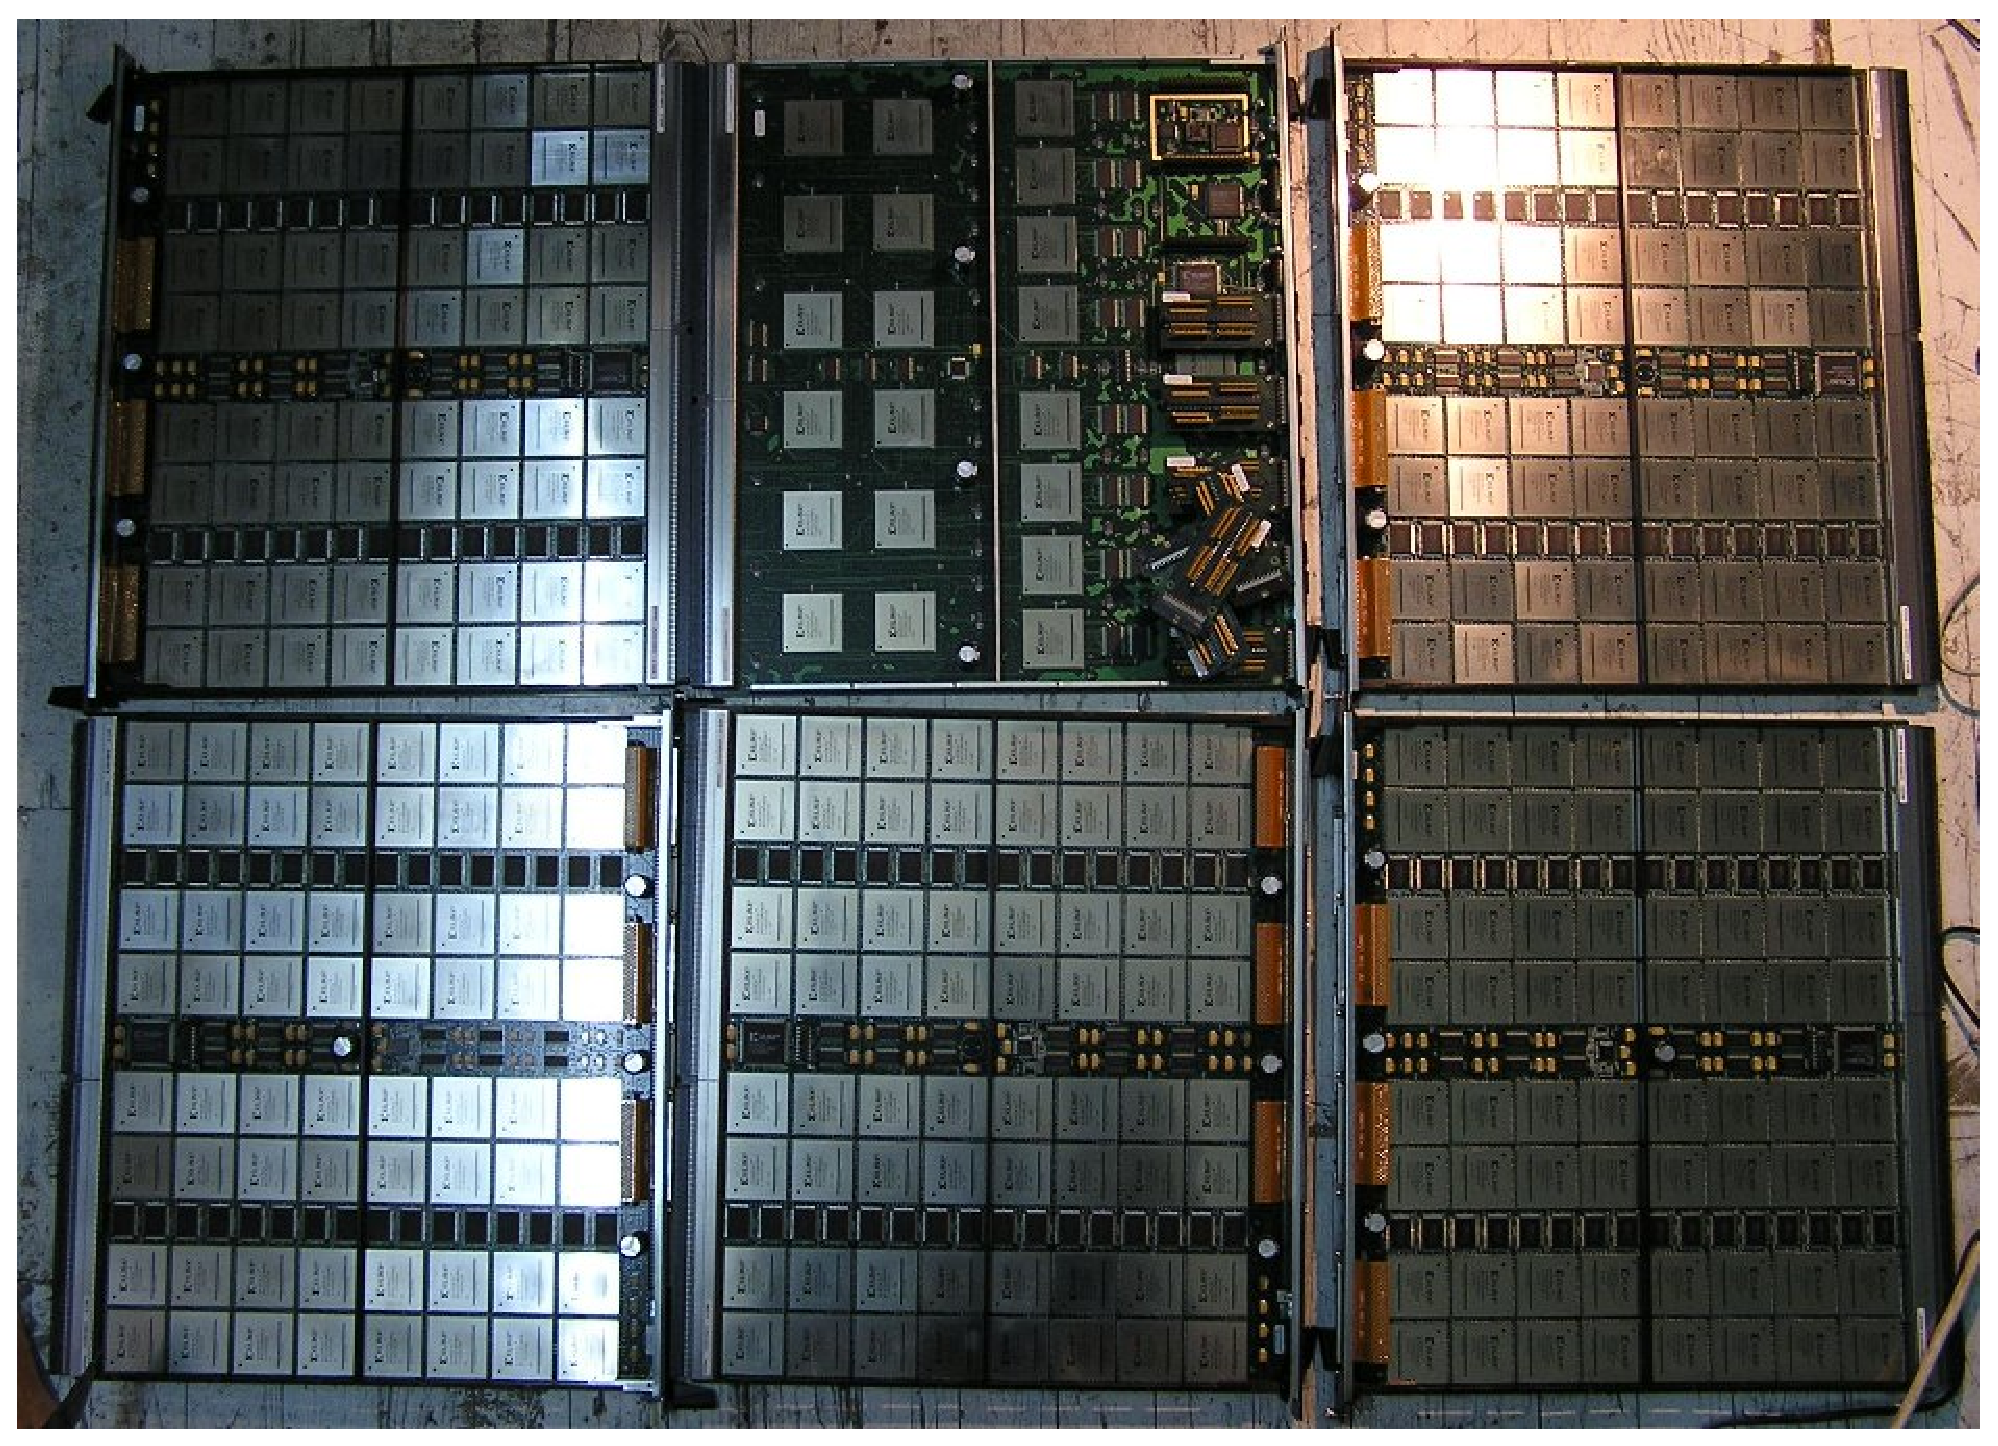
\includegraphics[height=95mm]{ikosboards.eps}
\caption{FPGA boards of the Ikos Pegasus ASIC emulator (ca. 1999)}
\label{fig:ikos}
\end{figure}

But today, the cost of fast high-density FPGAs is falling and these devices are becoming available to the general public. For an example of this trend, I would mention the Ikos Pegasus application specific integrated circuit (ASIC) emulator, whose insides are depicted in Figure~\ref{fig:ikos}. The CPU core used in the system-on-chip described in this thesis occupies alone 60\% of the resources of one of the XC4036XL FPGAs of this device, and runs at 30MHz. The Ikos Pegasus was a state-of-the-art device a decade ago. It consumes up to 3 kilowatts of power, weights dozens of kilos and costed the equivalent of several millions of SEK. The same CPU core now occupies about 15\% of a modern FPGA costing less than 500 SEK, where it runs in excess of 100MHz.

This evolution makes it possible to implement complex high-performance system-on-chips (SoC) that can be modified and improved by anyone, thanks to the flexibility of the FPGA platform.

This master thesis introduces Milkymist~\cite{milkymist}, a fast and resource-efficient FPGA-based system-on-chip designed for the application of rendering live video effects during performances such as concerts, clubs or contemporary art installations. Such effects are already popularized by artists known as ``video jockeys'', or ``VJs''.

Besides the fact that this is an interesting, creative and popular application, it is also demanding in terms of computational power and memory performance. It would make Milkymist a proof that high performance open source system-on-chip design is possible in practice; with a view to help, foster and catalyze similar ``open hardware'' initiatives. As the Milkymist system-on-chip is entirely made of synthesizable Verilog and, for the most part, released under the GNU GPL, its code can be re-used by other open hardware projects.

Meeting the performance constraints while still using cheap and relatively small FPGAs is perhaps the most interesting and challenging technical point of this project, and it could not be done without considerable work in the field of computer architecture. This is what this master thesis covers.

\section{Background}
MilkDrop~\cite{milkdrop} is a popular open source video synthesis framework that was originally made to develop visualization plugins for the Winamp audio player. People have since then ported MilkDrop to many different platforms and made it react to live events, such as captured audio or movements of a WiiMote remote control.

The idea behind the Milkymist project is to implement an embedded video synthesis platform on a custom open source system-on-chip that is based on the same rendering principle of MilkDrop, but with more control interfaces and features.

\begin{figure}[htp]
\centering
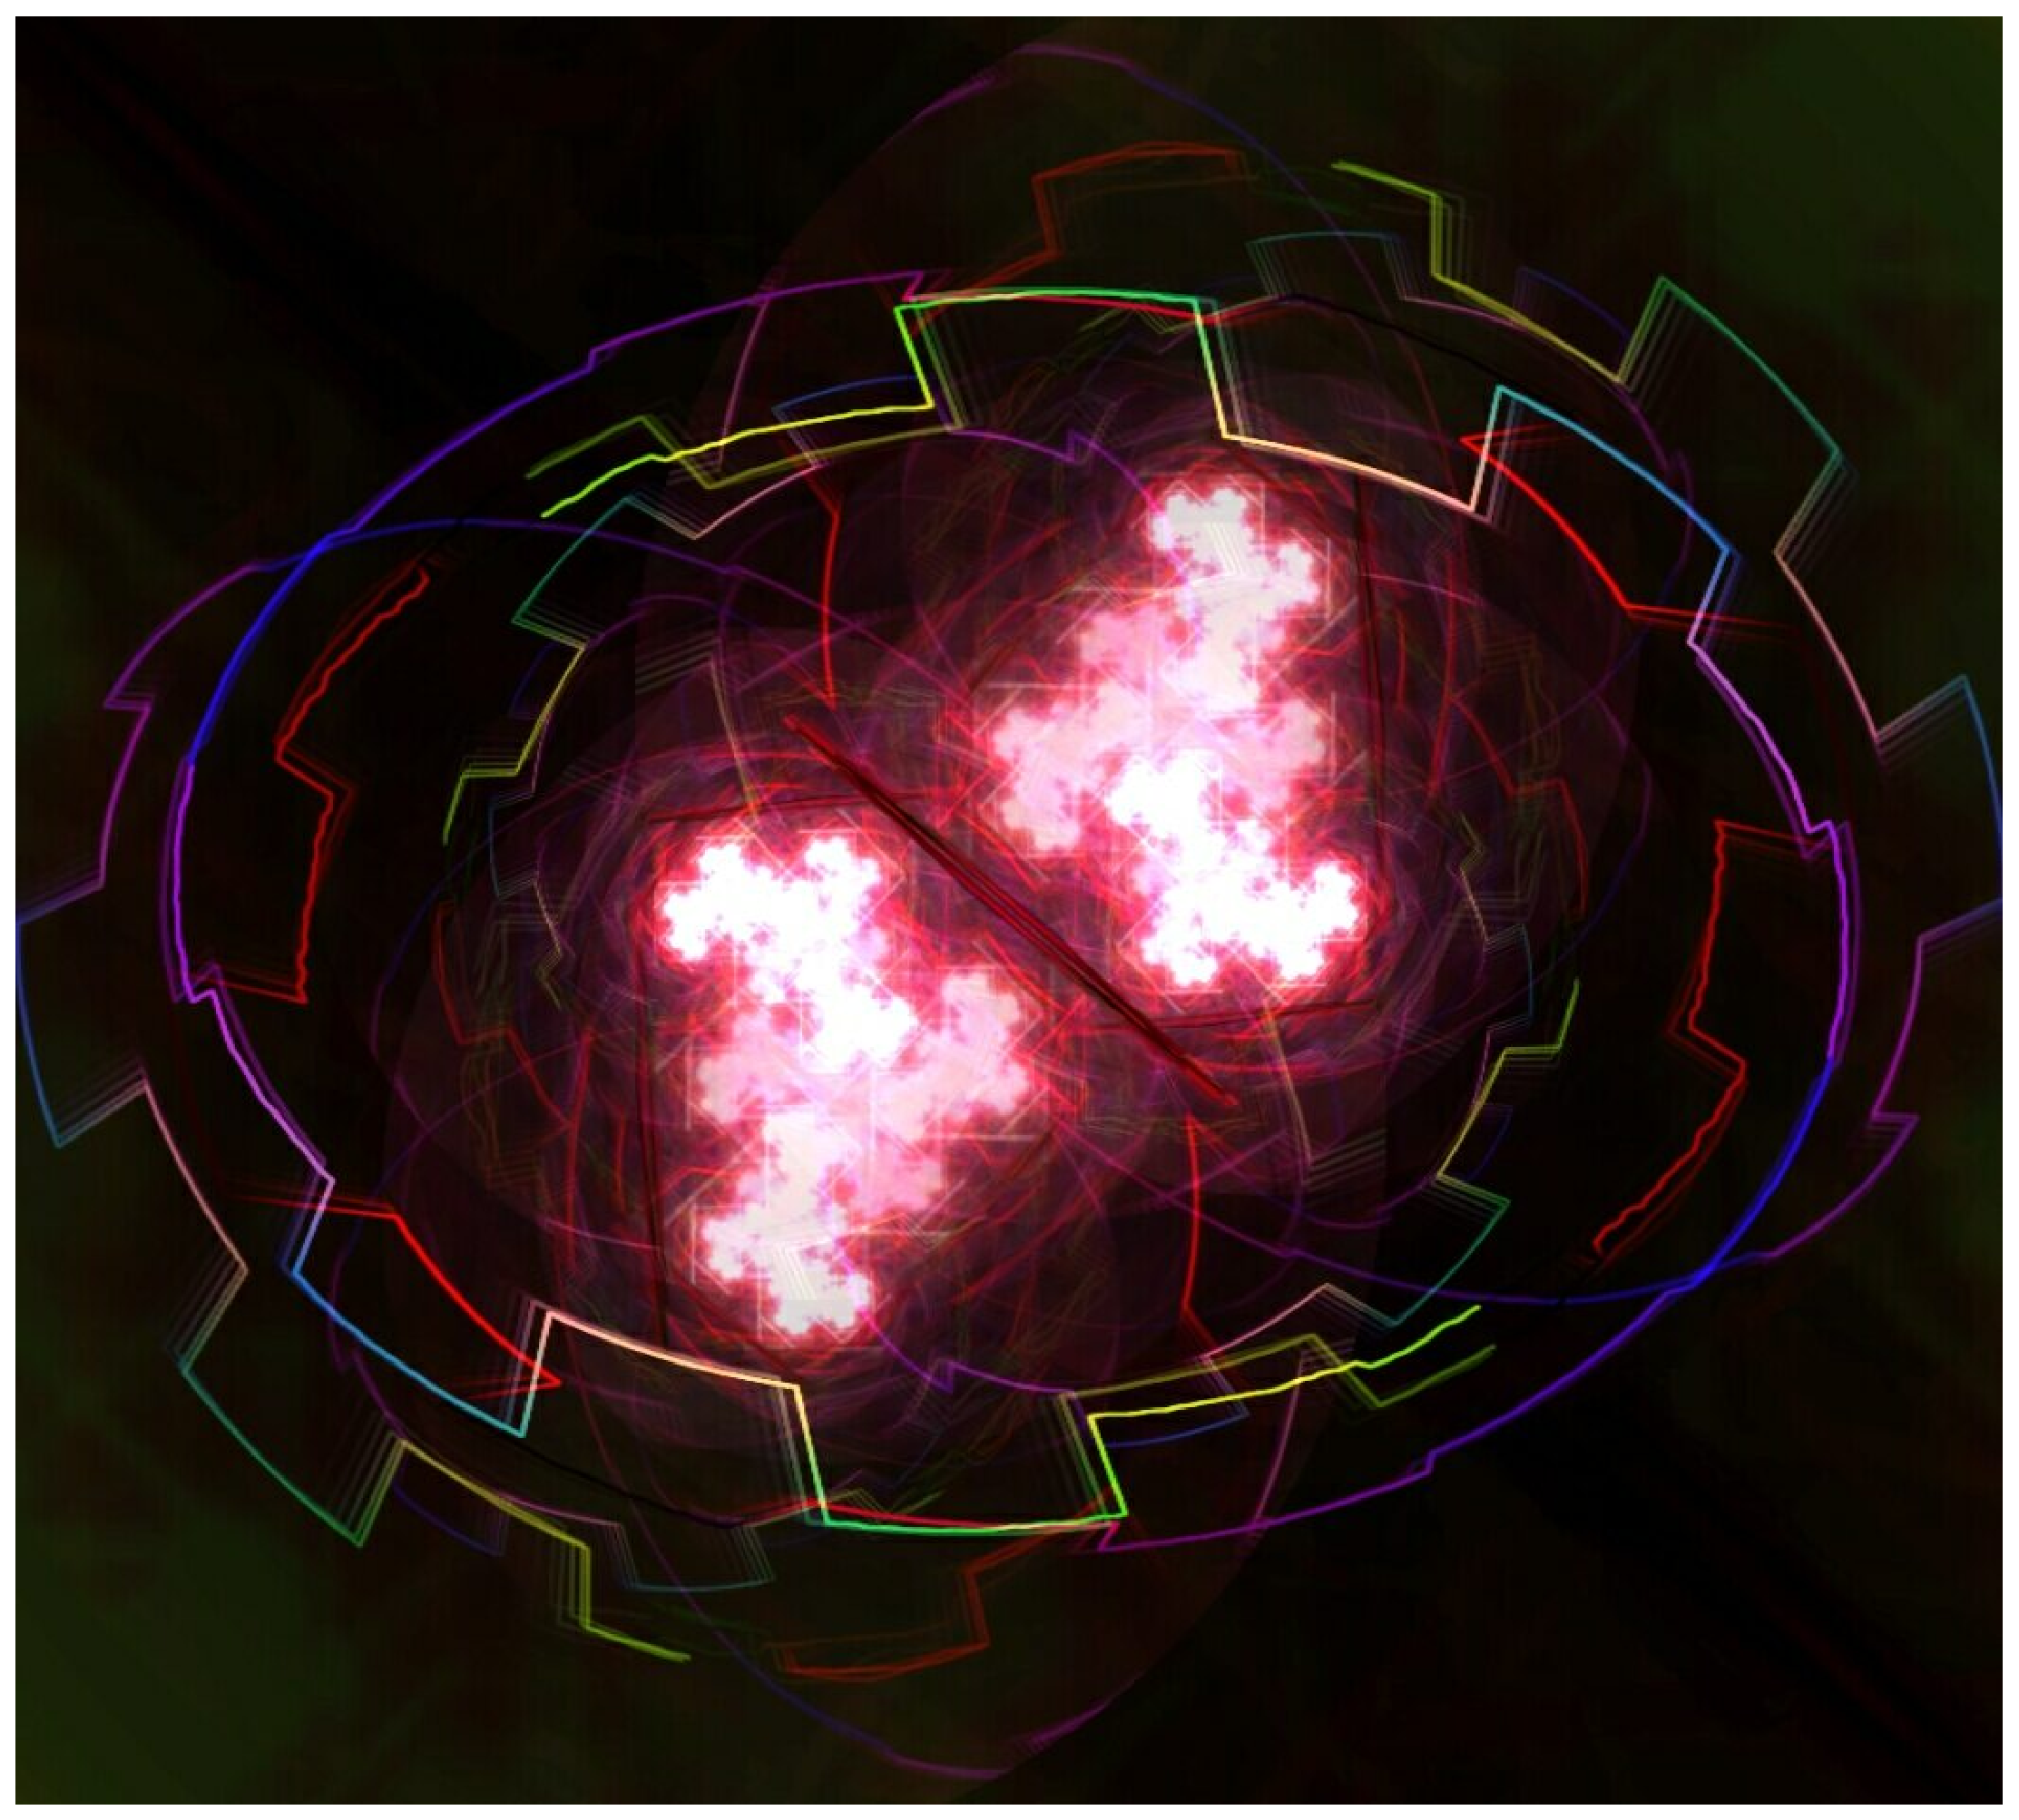
\includegraphics[height=65mm]{milkdrop2.eps}
\caption{Sample video frame from the MilkDrop visual synthesizer.}
\label{fig:milkdrop}
\end{figure}

\section{Problem statement}
TODO

\chapter{Memory system}
\chapter{Software execution environment}
\section{Description}
Linux has been ported to the Milkymist SoC (Figure~\ref{fig:linux}). Since this is a community effort, the details will not be covered in this master thesis. Still, this demonstrates the capability of the platform to run complex software.

\begin{figure}[htp]
\centering
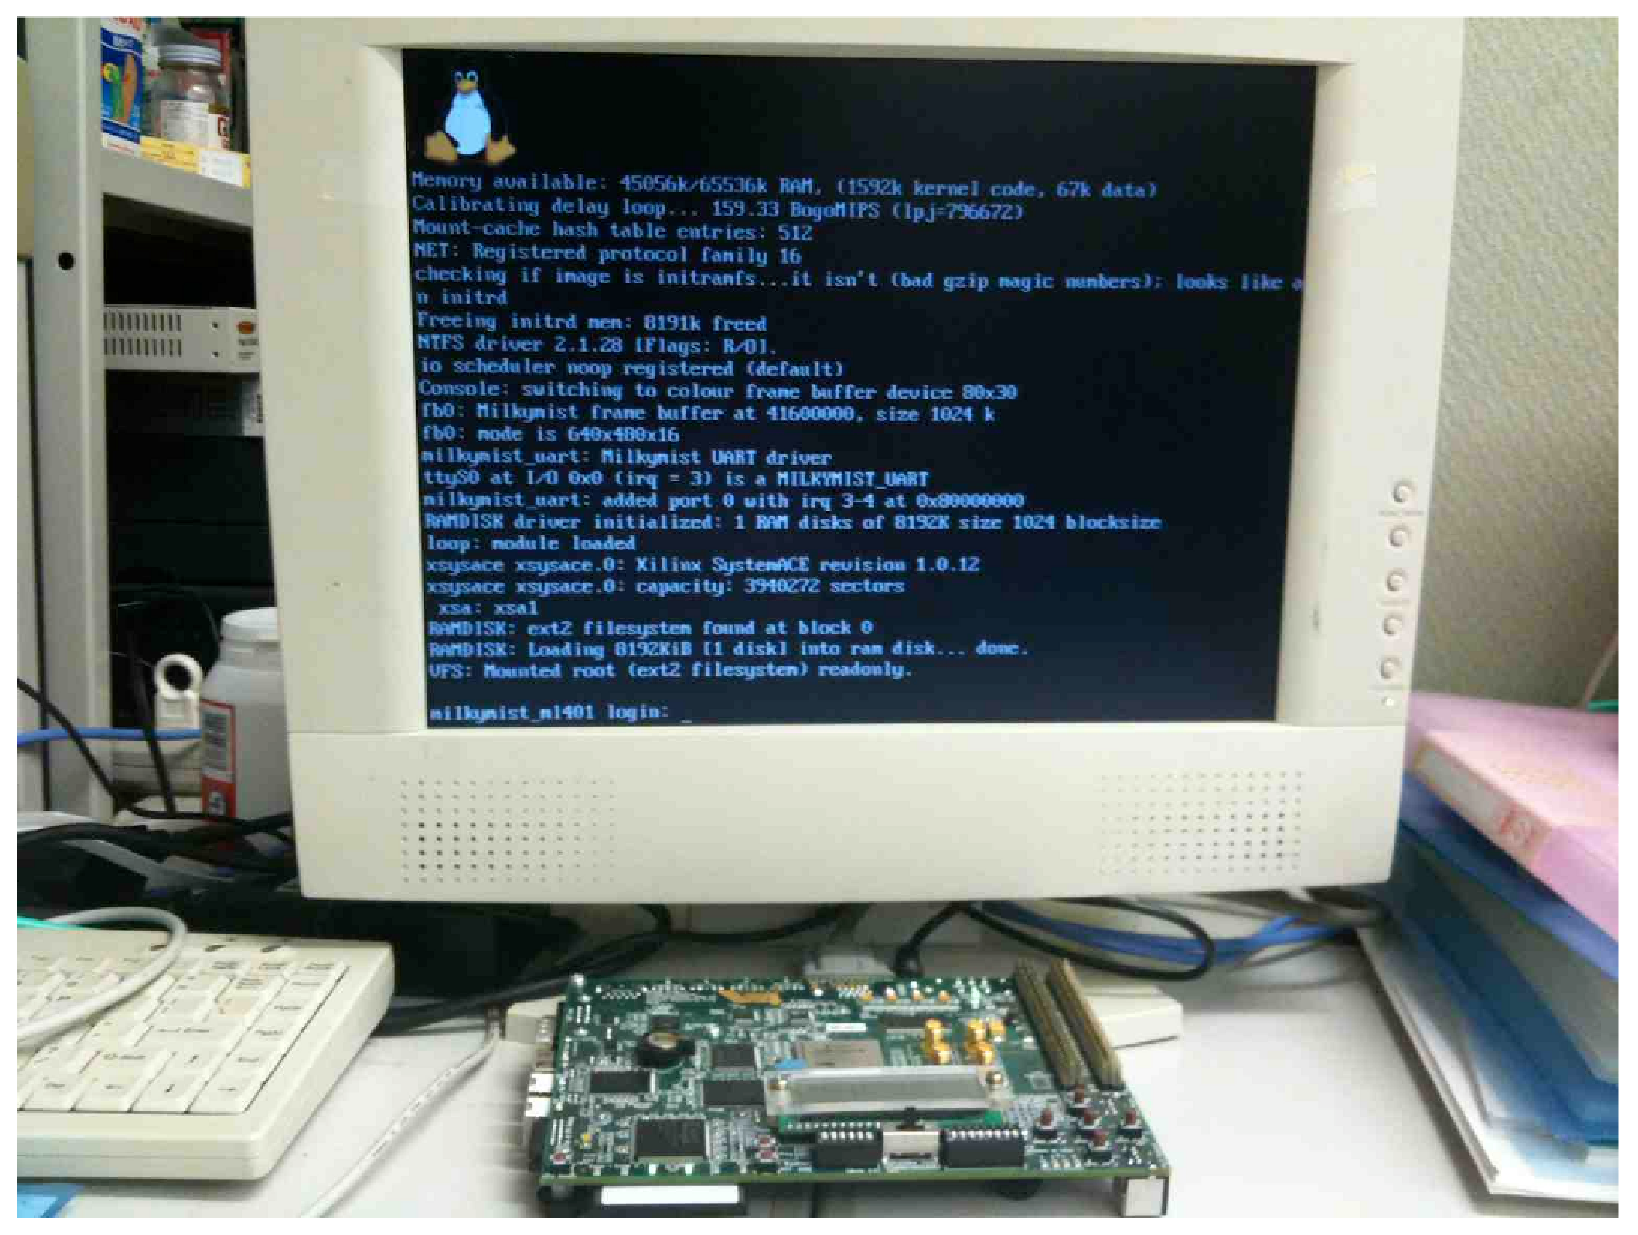
\includegraphics[height=92mm]{linux.eps}
\caption{Linux booting on the Milkymist SoC.}
\label{fig:linux}
\end{figure}
\section{Tuning and benchmarking}

\bibliography{thesis}{}
\bibliographystyle{plain}

\end{document}
